\documentclass[11pt]{article}
\usepackage[utf8]{inputenc}
\usepackage{graphicx}
\usepackage{float}
\usepackage{natbib}
\linespread{1.5}


\title{CMEE Miniproject - Compare the Model Fitting Quantified by LogisticGrowth Data}
\author{Jintao Lu}
\date{December 2022}

\begin{document}
\maketitle
\rule{\textwidth}{4pt}

\begin{abstract}
Models are increasingly essential tools for understanding complex data, factors, and further projecting future trends during research in ecology and evolution. Numerous models have been developed thus far, all of which are attempting to fit the experimental data as best they can. The primary techniques for testing and learning are the linear model and the non-linear model\citep{levins1966strategy}. By fitting the identical growth rates data, two different linear models and two different non-linear models are compared in this study. According to this, the Gompertz model fit the majority of situations the best, while the logistic model fit the log data scale the best.

\end{abstract}

\section{Introduction}
Since the researcher's perspective on the microorganism, the growth rates have been the emphasis. The microorganism is simple to grow and study in the lab, in contrast to the slow growing period of a typical species. We use them to examine population change and growth rate in part because of this. Additionally, we could regulate the community by inputting various external parameters like temperature and humidity, all of which have an impact on the population's rate of growth and carrying capacity\citep{johnson2004model}. The model fitting is a technique for dealing with messy data and looking for patterns. The simplest mathematical approach, the basic linear method, is initially used to try and fit the data. However, it was clear that the straight line could only roughly accommodate the variable data. Therefore, advanced linear models such as quadratic and cubic models are prone to fitting the data. There are still alternative ways to fit data, though. Given that a variety of factors, including temperature and food, have an impact on species' populations. The non-linear models with parameters would suit the growth rate data more precisely\citep{bolker2013strategies}.
In order to evaluate four models in this study, I prepared a total of 285 pieces of data. Simple linear models and quadratic models are two linear models, while logistic models and additional gompertz models are two non-linear models. The goal is to determine which model best fits the data on growth rates. Additionally, using a normal or log scale for the environment could help the data fit more accurately.

\section{Method}

\subsection{language use and packages}
In order to help organise the data and handle the model fitting, I use shell scripts, Python 3, and R, along with the tools that go with them. The "Pandas" library in Python 3 is used to first restructure the raw data. The "minpack.lm" and "AICcmodavg" packages in the R language are then used to help fit the non-linear model and calculate the AIC with the AICc. Additionally, I utilise the "plyr" and "dplyr" packages to reshape and clean up the data before, during, and after model fitting. The "ggplot2" and "ggthemes" programmes are configured to produce the graphs that aid in the analysis of the data and outcomes.

\subsection{data preparation}
The "logisticGrowthMetaData.csv" file revealed that PopBio and Time are the factors that I need to fit with models after storing the necessary packages. With the exception of these two components, all of the data were then concatenated in Python 3 before being split into 285 CSV files to store the sorted data.

\subsection{models introduction}
The first model is linear regression, the easiest way to fit the data, which formula is: 
$$
y = \beta_0 + \beta * x + \epsilon
$$
In addition, more complex linear model is also set for fitting which is the quadratic model:
$$
y = c + b *x + a* x^2
$$
Non-linear models are carrying with parameters, therefore they might be closer to the ideal fitting when used. The traditional logistic model(equation), which is the first non-linear model, is as follows:
$$
N_t= \frac{N_0 *K * e^[r*t]}{K + N_0(e^[r*t] -1)}
$$
where Nt is PopBio number at time t, N0 is initial PopBio number, r is maximum growth rate and K is carrying capacity.

In addition to the conventional logistic model, the Gompertz model, which would also fit with the data in a high fitness, is frequently used in the literature to model bacterial growth. The Gompertz model equation is as follows:
$$
log(N_t)=N_0 +(N_max-N_0)*e^{{-e}^{{r_{max}* exp(1) *{\frac{t_{lag}-t}{(N_{max}-N_0)*log(10)}+1}}}}
$$


\subsection{model fitting procedure}
Remove the three files "15.csv," "25.csv," and "26.csv" from the data set because they would halt the subsequent nlsLM run. Use "try()" in the "Model fitting" R script to disregard incorrect fits and continuous next model fitting that result in "NA" or "inf." Next, determine AIC and AICc values for various scales. While one example fitting was plotted out and the AIC with AICc results were filtered and plotted by pie chart in the "Plot analysis" R script.

\subsection{model comparison: AIC and AICc calculation, normal and log scale}
An estimator of prediction error and consequently of the relative quality of statistical models for the data is the Akaike information criterion (AIC) value. In addition, because the sample size for the data set is tiny, the AICc value seems more appropriate for determining the outcomes and contrasting the various models. In addition, the data set contains hundreds of tiny 0.001 integers, thus the log scale is used to assist the model fit organically\citep{burnham2004multimodel}.

\subsection{ final step}
Finally, run with the "run miniproject.sh" script to simulate the whole workflow.

\section{Results}
\subsection{the model fitting example}
Here, I sorted a unique ID with the separate data and apply four models to fit it under normal and log scale. The fitting graph is shown below,\ref{fig.1.1}\ref{fig.1.2}:

\begin{figure}[H]
    \centering
    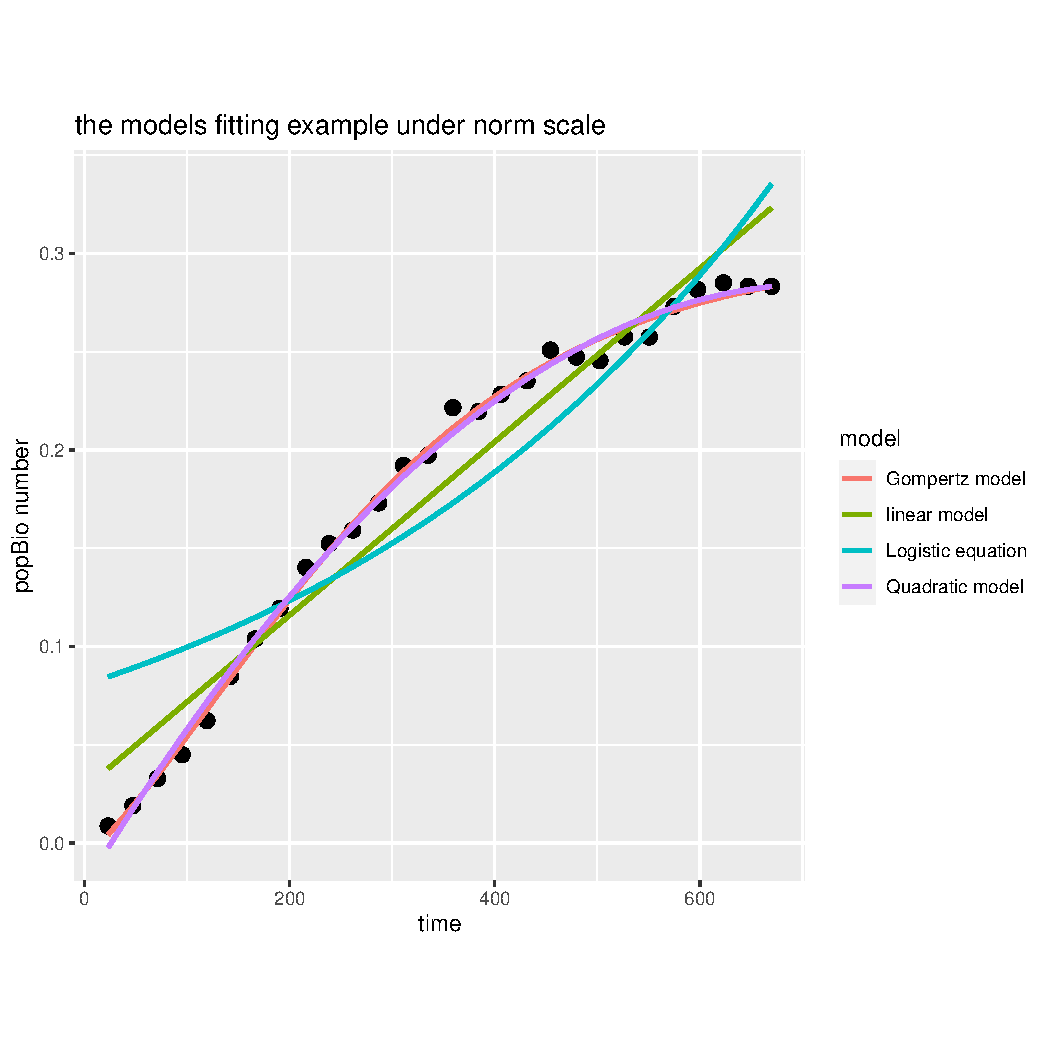
\includegraphics[scale=0.4]{example1.pdf}
    \caption{one example of model fitting to growth rate data}
    \label{fig.1.1}
\end{figure}

\begin{figure}[H]
    \centering
    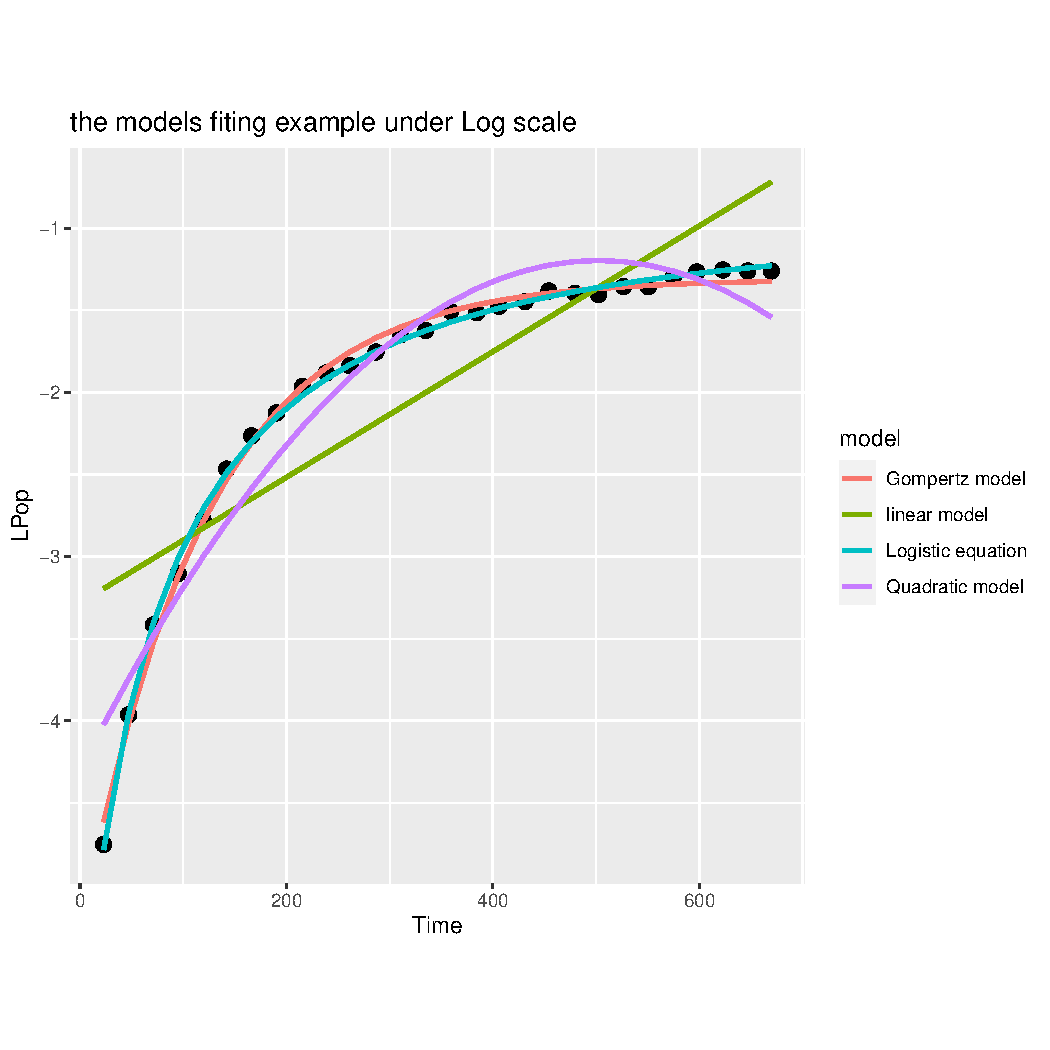
\includegraphics[scale=0.4]{example2.pdf}
    \caption{one example of model fitting to growth rate data}
    \label{fig.1.2}
\end{figure}

Given that they are close to the data trend, the quadratic and Gompertz models fit the data best under normal scale, while the logistic and linear models do not. The logistic and Gompertz models all fit the data well on the lower graph, which is a log scale; however, there is still a small amount of variation, and the quadratic and linear models do not.
\subsection{Pie chart distribution for the AIC and AICc values}
The following chart illustrates the overall AIC and AICc values percantage for each of the four scenarios:

\begin{figure}[H]
    \centering
    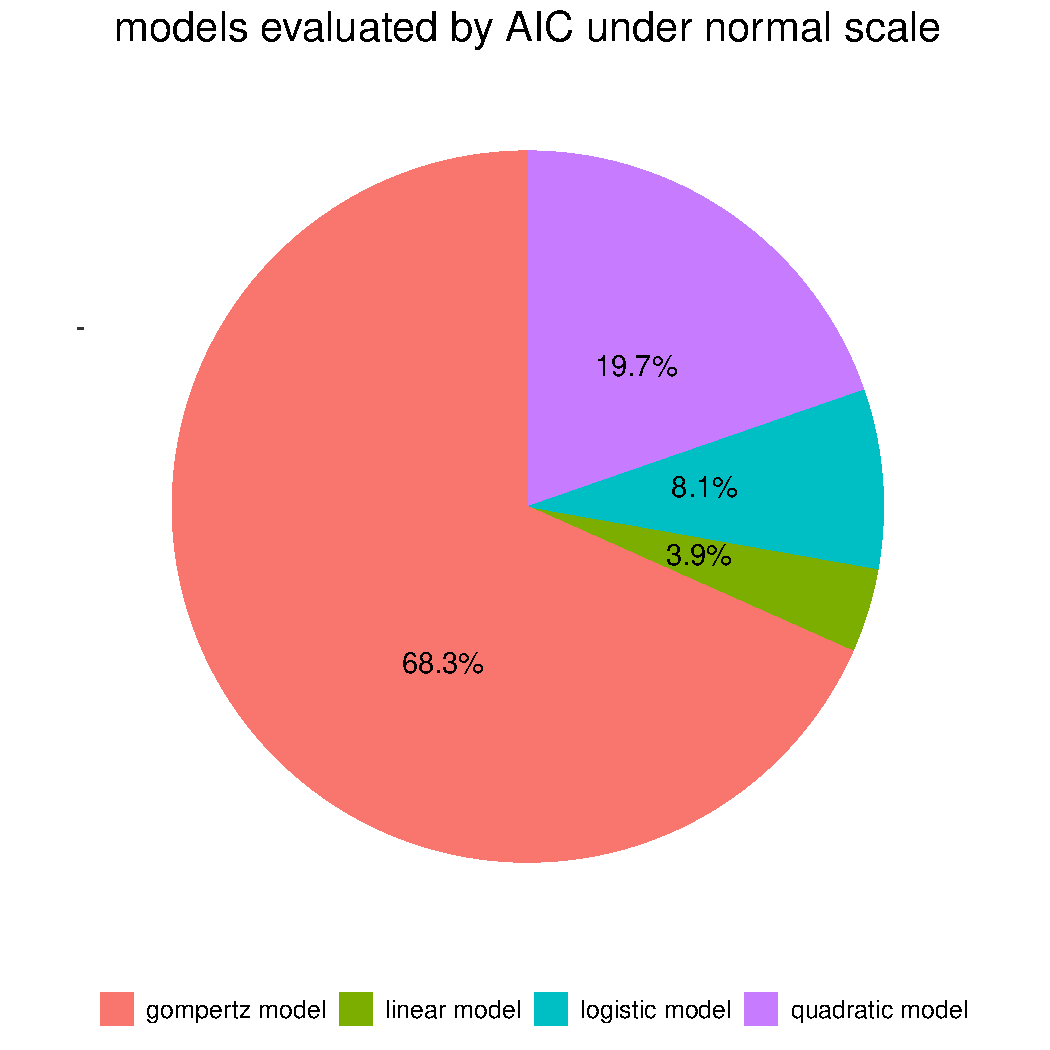
\includegraphics[scale=0.3]{AIC_norm.pdf}
    \caption{one example of model fitting to growth rate data}
    \label{fig.2}
\end{figure}

\begin{figure}[H]
    \centering
    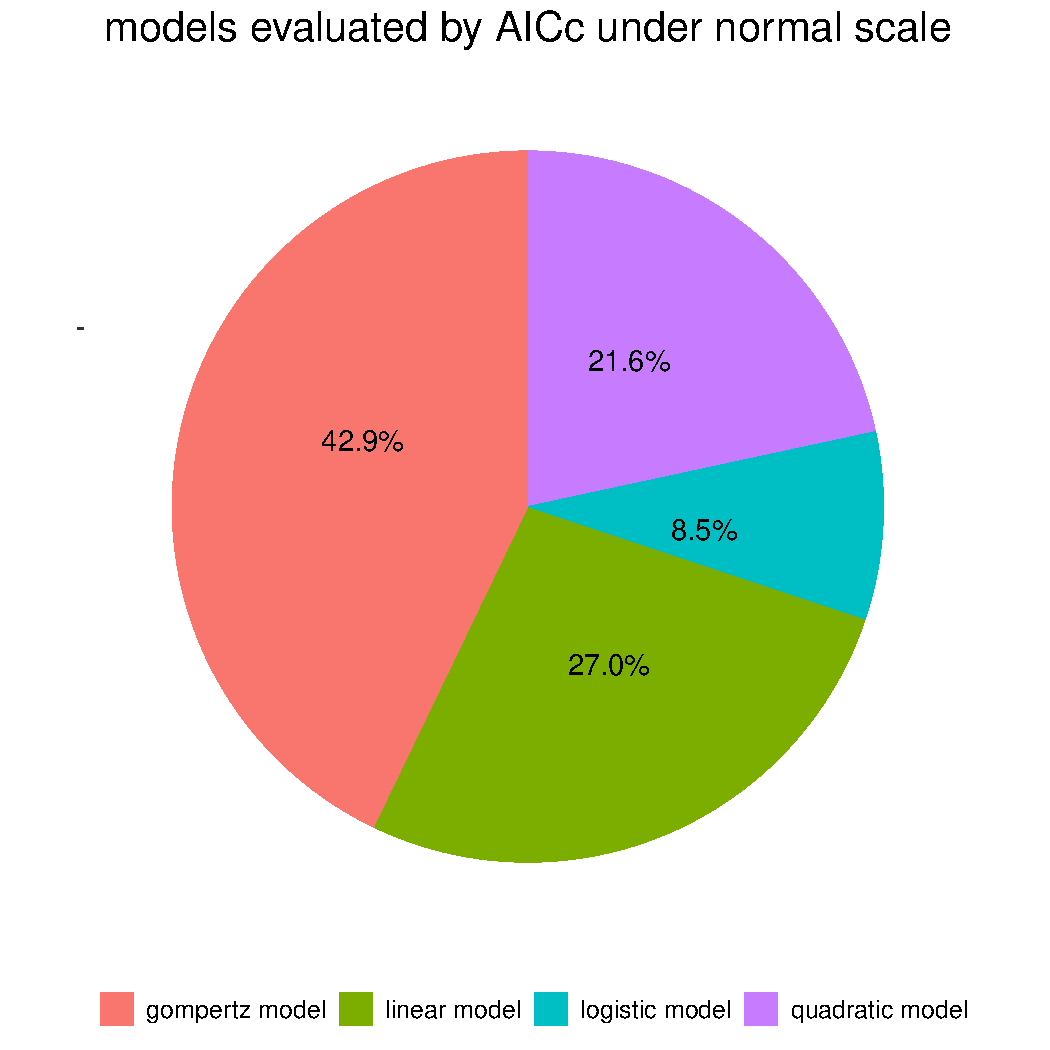
\includegraphics[scale=0.3]{AICc_norm.pdf}
    \caption{one example of model fitting to growth rate data}
    \label{fig.3}
\end{figure}

\begin{figure}[H]
    \centering
    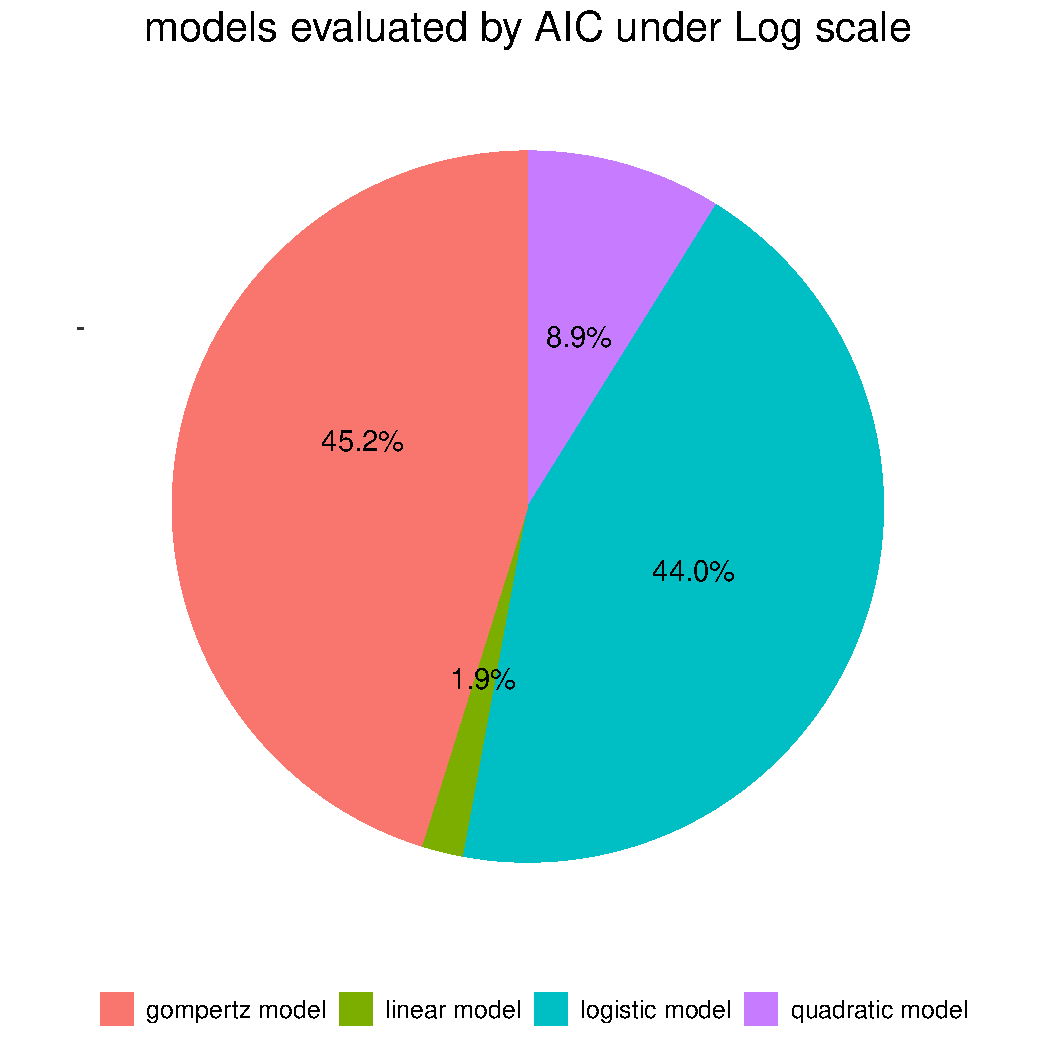
\includegraphics[scale=0.3]{AIC_Log.pdf}
    \caption{one example of model fitting to growth rate data}
    \label{fig.4}
\end{figure}

\begin{figure}[H]
    \centering
    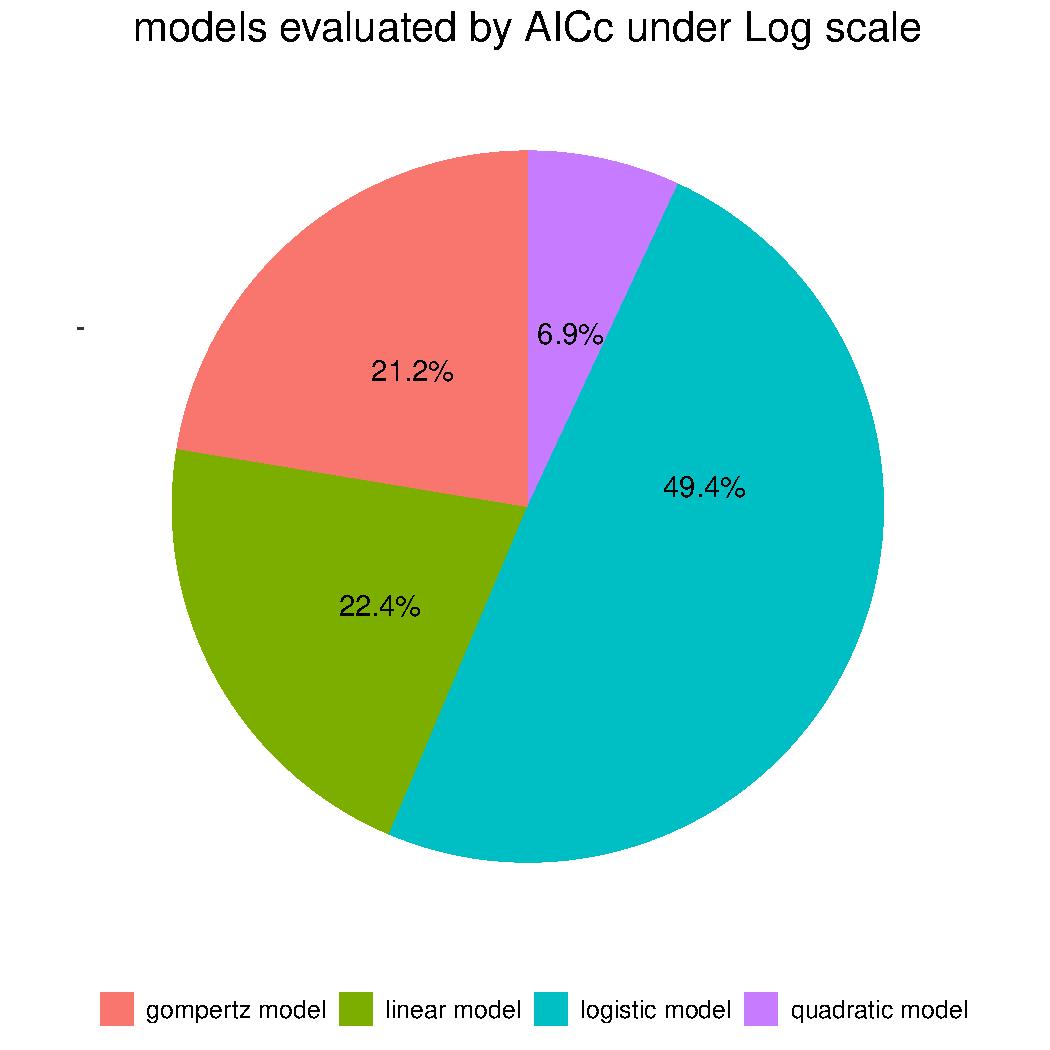
\includegraphics[scale=0.3]{AICc_Log.pdf}
    \caption{one example of model fitting to growth rate data}
    \label{fig.5}
\end{figure}

When compared to four pie charts, the gompertz model occupies the most amount in three of the charts, followed by the logistic model. The least is two linear models.
\subsection{Considering the Difference Between AIC and AICc}
Due to the AICc's limited sample computation design. The difference between them across all calculations is depicted in the graph below.

\begin{figure}[H]
    \centering
    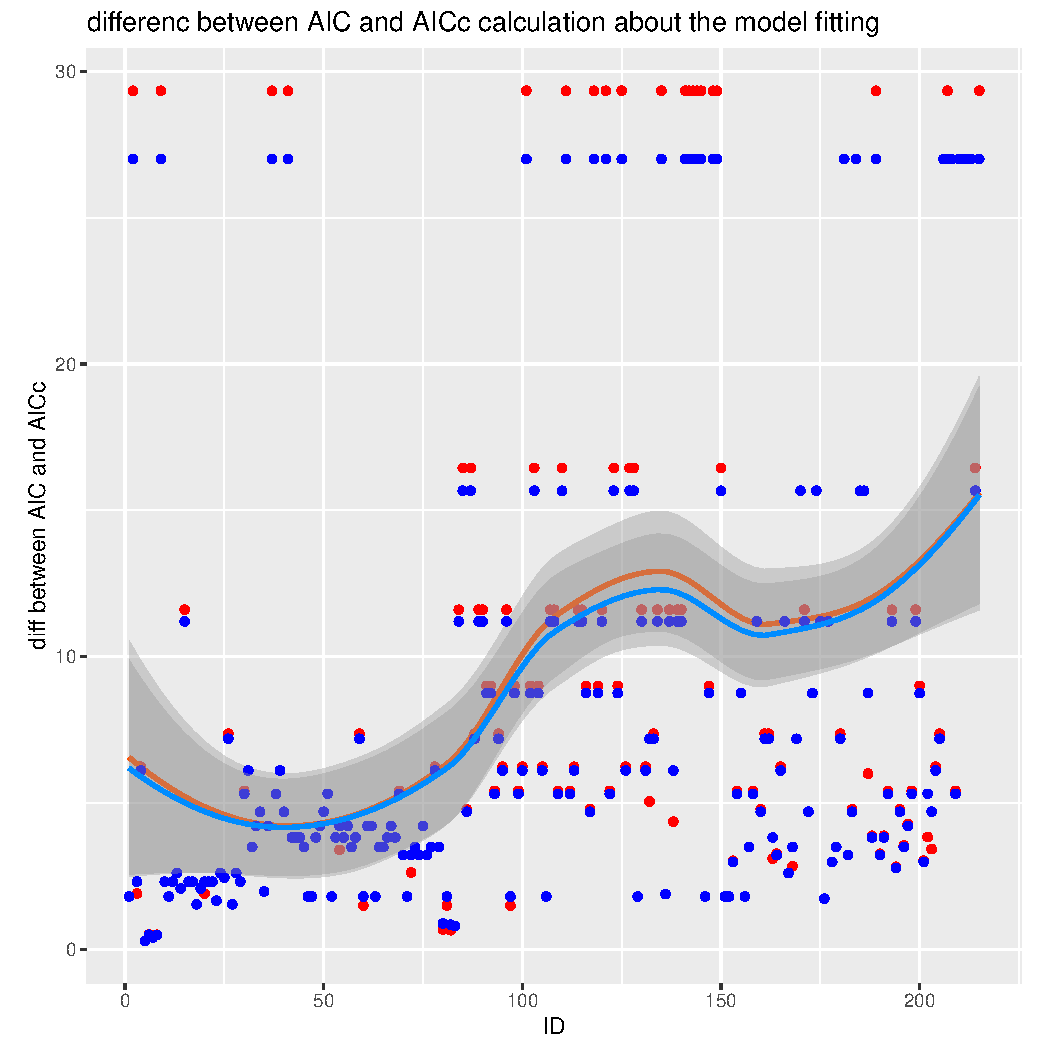
\includegraphics[scale=0.4]{difference_between_AICand AICc.pdf}
    \caption{one example of model fitting to growth rate data}
    \label{fig.6}
\end{figure}

All the scatter plot and the fitting lines indicate that these two value are closed that nearly difference existing.
\subsection{Consideration of data scales}
The box plots show that the AIC and AICc values have a higher density distribution in normal scale than in log scale, as shown in the graph below. The table also demonstrates that the standard deviation for data in the log scale is less than the norm, indicating higher data quality.

\begin{figure}[H]
    \centering
    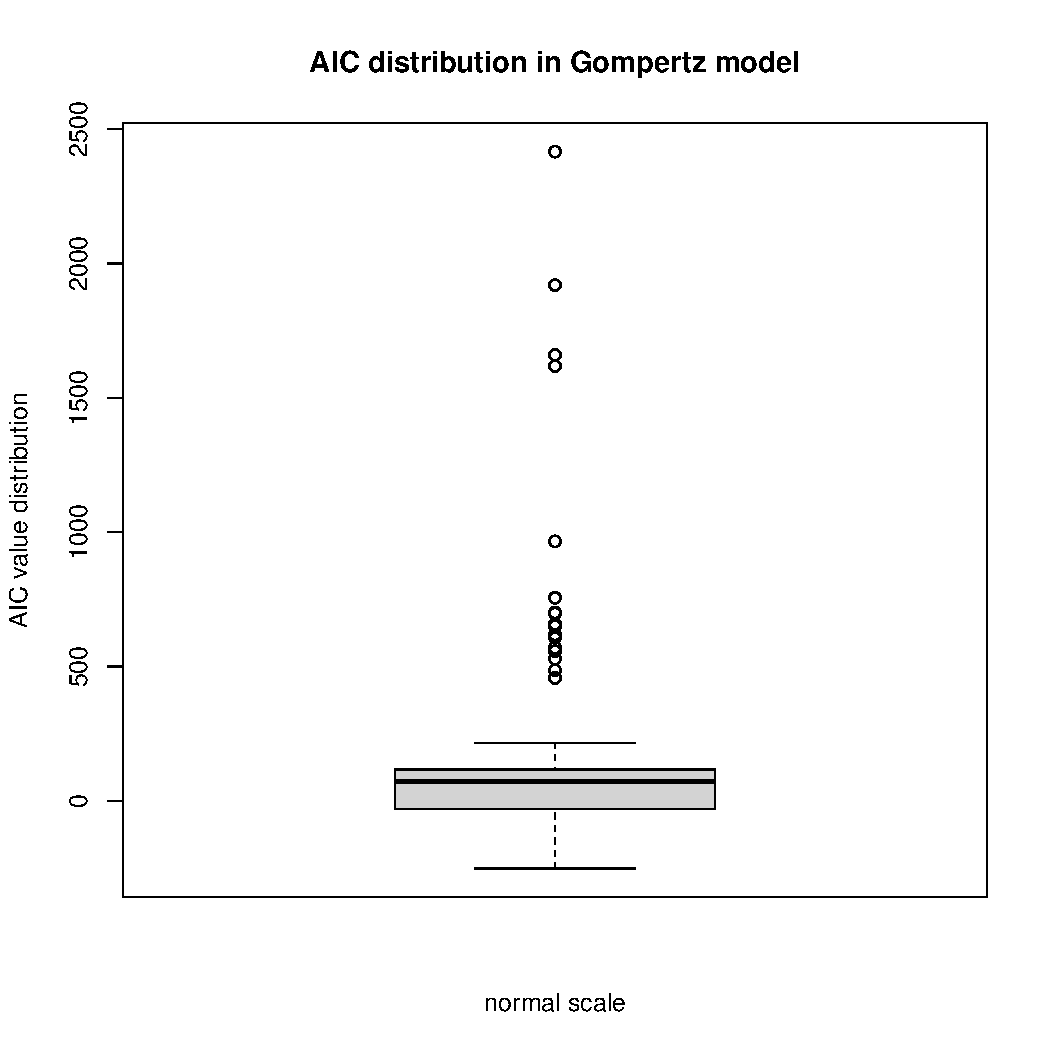
\includegraphics[scale=0.3]{GomAIC_norm.pdf}
    \caption{one example of model fitting to growth rate data}
    \label{fig.7}
\end{figure}

\begin{figure}[H]
    \centering
    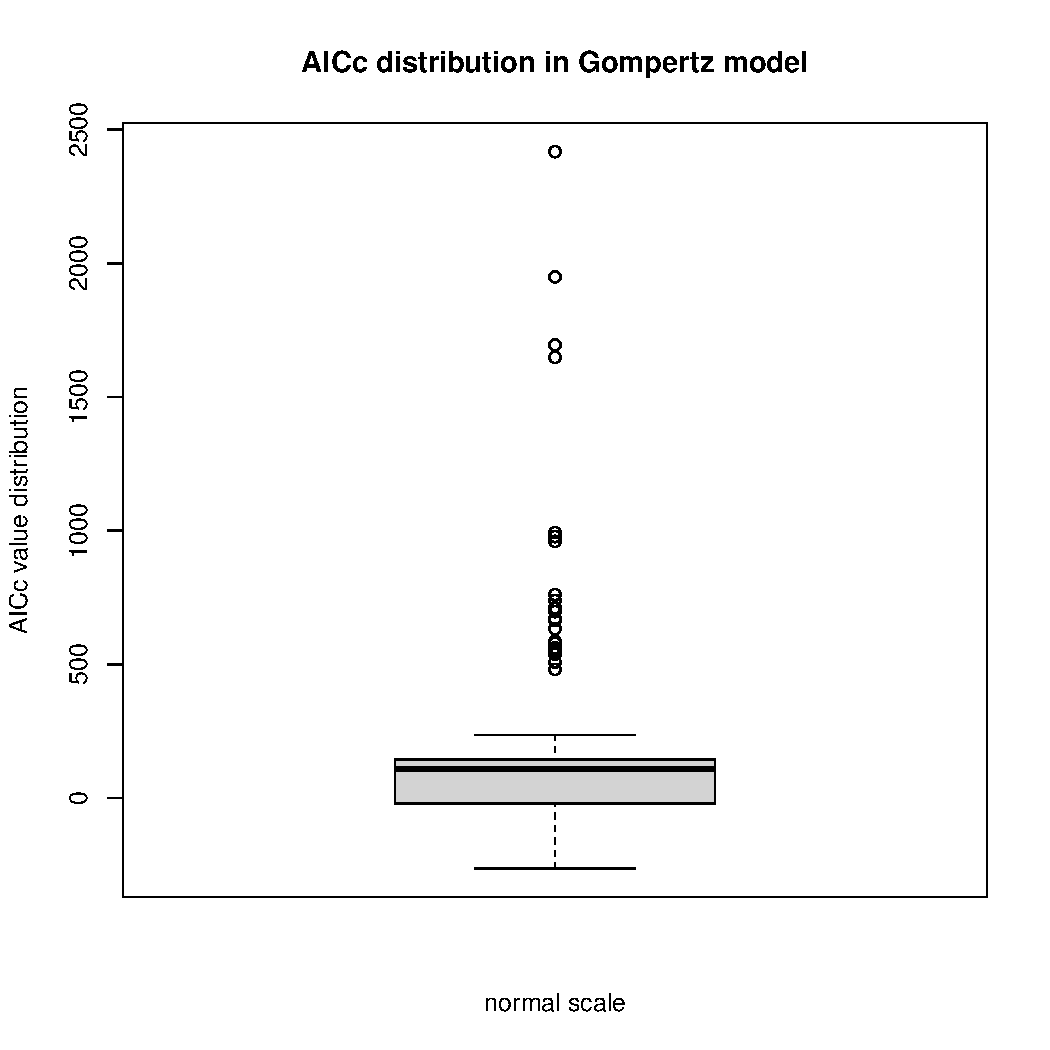
\includegraphics[scale=0.3]{GomAICc_norm.pdf}
    \caption{one example of model fitting to growth rate data}
    \label{fig.8}
\end{figure}

\begin{figure}[H]
    \centering
    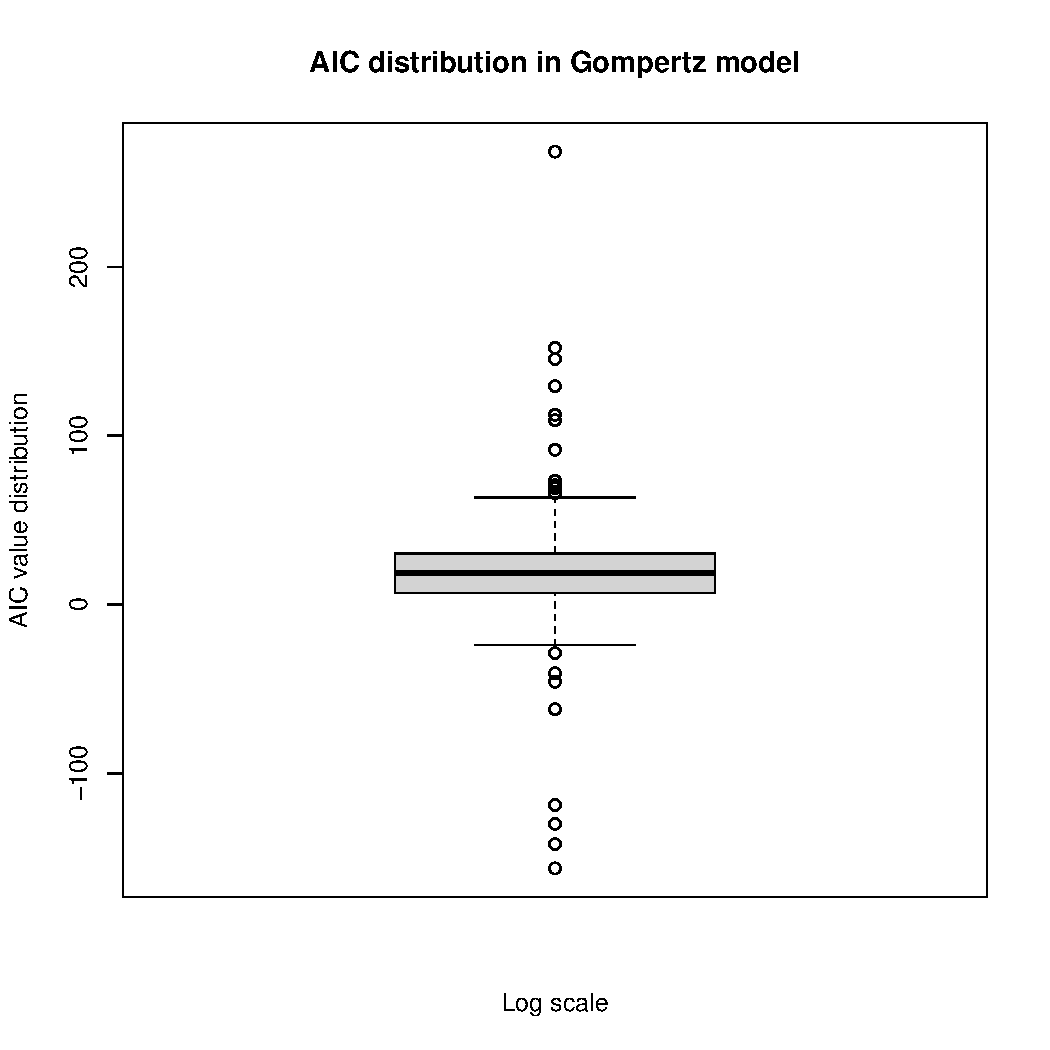
\includegraphics[scale=0.3]{GomAIC_Log.pdf}
    \caption{one example of model fitting to growth rate data}
    \label{fig.9}
\end{figure}

\begin{figure}[H]
    \centering
    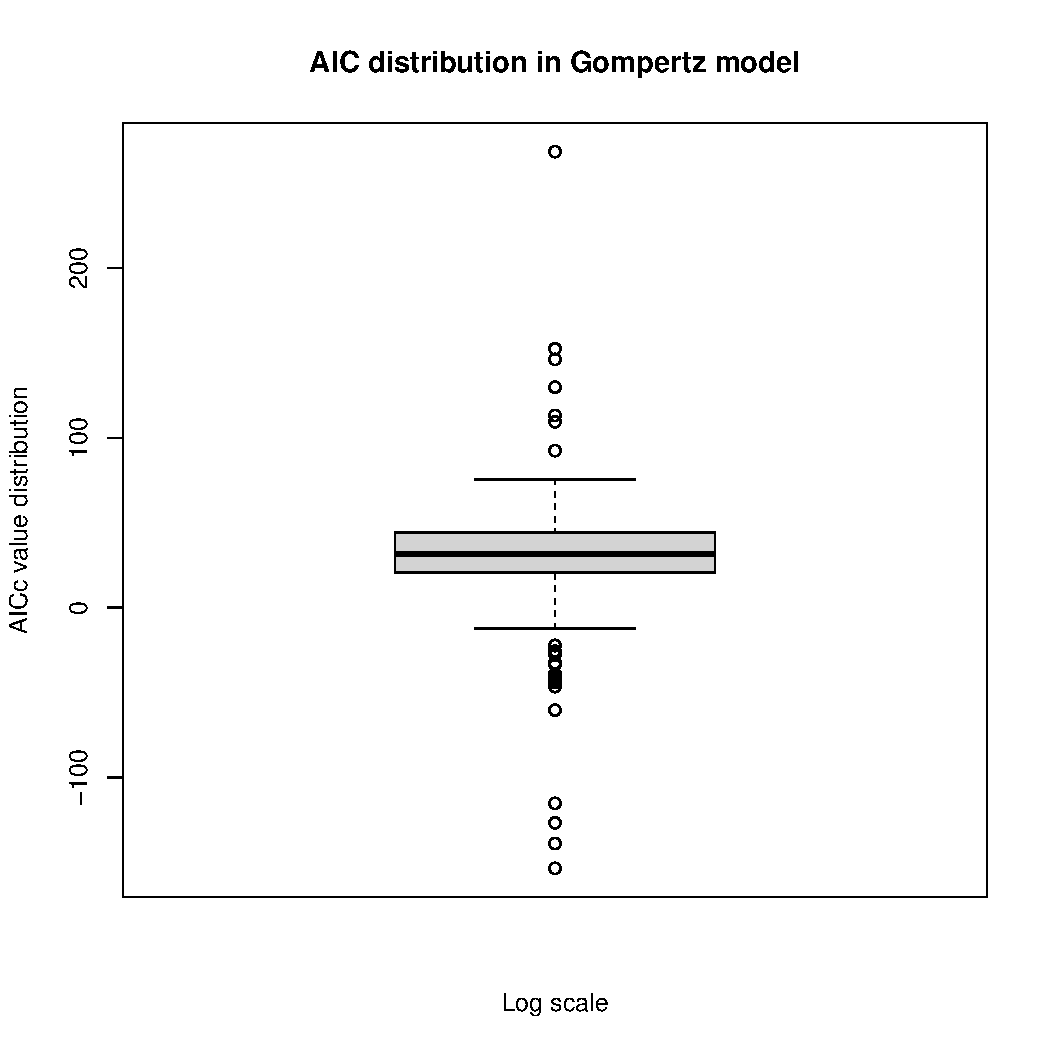
\includegraphics[scale=0.3]{GomAICc_Log.pdf}
    \caption{one example of model fitting to growth rate data}
    \label{fig.10}
\end{figure}

\begin{table}[H]
\caption{Standard deviation between AIC and AICc in the Gompertz model}
\label{tab:my-table}
\begin{tabular}{|l|l|l|l|l|}
\hline
                                                              & \begin{tabular}[c]{@{}l@{}}Gom\_norm\_\\ AIC\end{tabular} & \begin{tabular}[c]{@{}l@{}}Gom\_norm\_\\ AICc\end{tabular} & \begin{tabular}[c]{@{}l@{}}Gom\_Log\_\\ AIC\end{tabular} & \begin{tabular}[c]{@{}l@{}}Gom\_Log\_\\ AICc\end{tabular} \\ \hline
\begin{tabular}[c]{@{}l@{}}standard \\ deviation\end{tabular} & 294.7931                                                  & 313.585                                                    & 58.7459                                                  & 71.417                                                    \\ \hline
\end{tabular}
\end{table}

\section{Discussion}
According to the \ref{fig.6} above, even if the sample size is generally too small, the AIC and AICc values could be equally taken into account when determining which model fits the data the best. It indicates that I use AIC and AICc as criteria for model fitting. When comparing the data under the log scale and the norm, the data under the log scale is less fluctuated , which is more relied upon to support the conclusions\citep{burnham2004multimodel}. Additionally, the box plots in \ref{fig.7}\ref{fig.8}\ref{fig.9}\ref{fig.10}demonstrate that the calculation value is of higher quality under the log scale, and the standard deviation judgement in \ref{tab:my-table} further supports this claim. A convenient method for converting a variable with a high skewness into a dataset with a more normal distribution is logarithmic transformation. The likelihood of making errors may also be skewed negatively when modelling variables with non-linear connections. Theoretically, when generating a forecast, we want to make as little inaccuracy as possible while still keeping in mind that we shouldn't be overfitting the model\citep{claeskens2008model}. When there are too many dependent variables involved, the dataset is overfitted, making it impossible to generate a reliable forecast. By changing the distribution of the features to a more typically shaped bell curve, using the logarithm of one or more variables enhances the model's fit. So I made the decision to think about the log scale environment first. Overall, I draw the conclusion from the pie charts that the Gompertz model fits the data the best overall, while the logistic model performed best under log scale\citep{verwijst1991logarithmic}.
Additionally, there are some restrictions in place. One is that I used the "try" function during coding to avoid model fitting because it was challenging to obtain the appropriate "r-initial" value. This resulted in many "NA" and "inf" values, which largely occurred in non-linear model fitting. As a result, it's possible that the pie chart's representation of the logistical proportion is inaccurate. AIC and AICc values calculated under the log scale may be negative in relation to the equation, which would potentially affect the outcomes, is another problem.
In conclusion, the Gompertz model fit the data the best overall, while the logistic model fit the data the best when using log scale.

word count:1399

\bibliographystyle{agsm}
\bibliography{Mybib}

\end{document}





